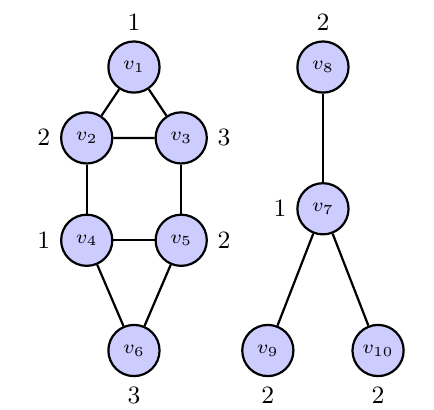
\begin{tikzpicture}[
  baseline=0pt,
  scale=1,
  vnode/.style={circle, draw=black, fill=blue!20, thick, inner sep=0pt, minimum size=6.5mm},
  edge/.style={thick, draw=black},
  clabel/.style={font=\small, color=black}
]
  % Se amplía xmin a -2.55 para añadir el medio carácter de margen izquierdo
  \useasboundingbox (-2.55,-2.2) rectangle (2.25,2.3);

  % --- COMPONENTE 1 ---
  \node[vnode, label={[clabel]above:$1$}] (v1) at (-1.2, 1.8) {$\scriptstyle v_1$};
  \node[vnode, label={[clabel]left:$2$}]  (v2) at (-1.8, 0.9) {$\scriptstyle v_2$};
  \node[vnode, label={[clabel]right:$3$}] (v3) at (-0.6, 0.9) {$\scriptstyle v_3$};
  \node[vnode, label={[clabel]left:$1$}]  (v4) at (-1.8, -0.4) {$\scriptstyle v_4$};
  \node[vnode, label={[clabel]right:$2$}] (v5) at (-0.6, -0.4) {$\scriptstyle v_5$};
  \node[vnode, label={[clabel]below:$3$}] (v6) at (-1.2, -1.8) {$\scriptstyle v_6$};

  \draw[edge] (v1) -- (v2) -- (v3) -- (v1);
  \draw[edge] (v2) -- (v4);
  \draw[edge] (v3) -- (v5);
  \draw[edge] (v4) -- (v5);
  \draw[edge] (v4) -- (v6);
  \draw[edge] (v5) -- (v6);

  % --- COMPONENTE 2 ---
  \node[vnode, label={[clabel]left:$1$}]  (v7)  at (1.2, 0.0) {$\scriptstyle v_7$};
  \node[vnode, label={[clabel]above:$2$}] (v8)  at (1.2, 1.8) {$\scriptstyle v_8$};
  \node[vnode, label={[clabel]below:$2$}] (v9)  at (0.5, -1.8) {$\scriptstyle v_9$};
  \node[vnode, label={[clabel]below:$2$}] (v10) at (1.9, -1.8) {$\scriptstyle v_{10}$};

  \draw[edge] (v7) -- (v8);
  \draw[edge] (v7) -- (v9);
  \draw[edge] (v7) -- (v10);
\end{tikzpicture}
